\begin{frame}[c]{}

\centering
\huge
Lecture 5:\\
Hyperparameter Optimization using Evolutionary Algorithms
\end{frame}
%----------------------------------------------------------------------
%----------------------------------------------------------------------
\begin{frame}[c]{Where are we? The big picture}

\begin{itemize}
	\item Introduction
	\item Background
	\begin{itemize}
		\item Design spaces in ML
		\item Evaluation and visualization
	\end{itemize}
	\item [$\to$] Hyperparameter optimization (HPO)
	\begin{itemize}
	  \item Bayesian optimization
	  \item [$\to$] Nature inspired algorithms/Evolutionary Algorithms (EAs) 
	  \item Speeding up HPO with multi-fidelity optimization
	\end{itemize}
	\item Pentecost (Holiday) -- no lecture
	\item Architecture search I + II
	\item Meta-Learning
	\item Learning to learn $\&$ optimize
	\item Beyond AutoML: algorithm configuration and control
	\item Project announcement and closing
\end{itemize}


\end{frame}
%----------------------------------------------------------------------
%----------------------------------------------------------------------

\begin{frame}{Evolutionary Algorithms}
Task: \hands [2min] \linebreak

Who knows evolutionary algorithms or nature inspired algorithms? If so, name some examples? 
\begin{center}
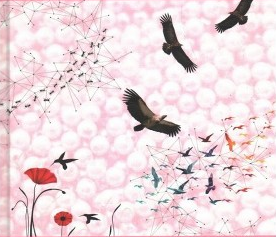
\includegraphics[width=0.5\textwidth]{new_images/EAs_02.png}
\end{center}

\end{frame}

\begin{frame}[c]{Learning Goals}

After this lecture, you will be able to \ldots

\begin{itemize}
	\item explain the basics of \alert{evolutionary algorithms}
	\item discuss the \alert{different types of evolutionary algorithms}
	\item efficiently tune \alert{HPO using evolutionary algorithms}
	\item discuss importance of \alert{evolutionary algorithms to solve many optimization problems}
\end{itemize}

\end{frame}
%----------------------------------------------------------------------
%----------------------------------------------------------------------

%\begin{frame}[c]{Optimization}
%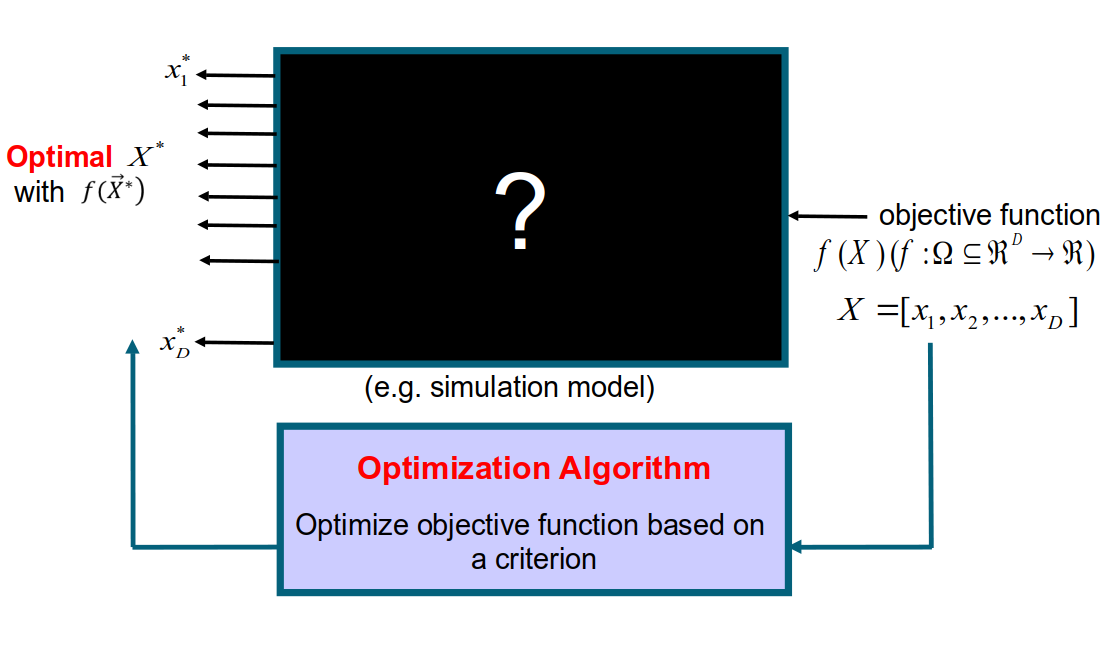
\includegraphics[width=1.0\textwidth]{new_images/optimization.png}
%\end{frame}

%-----------------------------------------------------------------------
\section{Basics of Evolutionary Algorithms}
%----------------------------------------------------------------------

\begin{frame}[c]{Nature Inspired Algorithms}
\begin{itemize}
	\item Nowadays, most new algorithms are nature-inspired, because they have been developed by drawing inspiration from nature
	\begin{itemize}
	    \item majority are based on some successful characteristics of biological system
	\end{itemize}
\end{itemize}
\centering
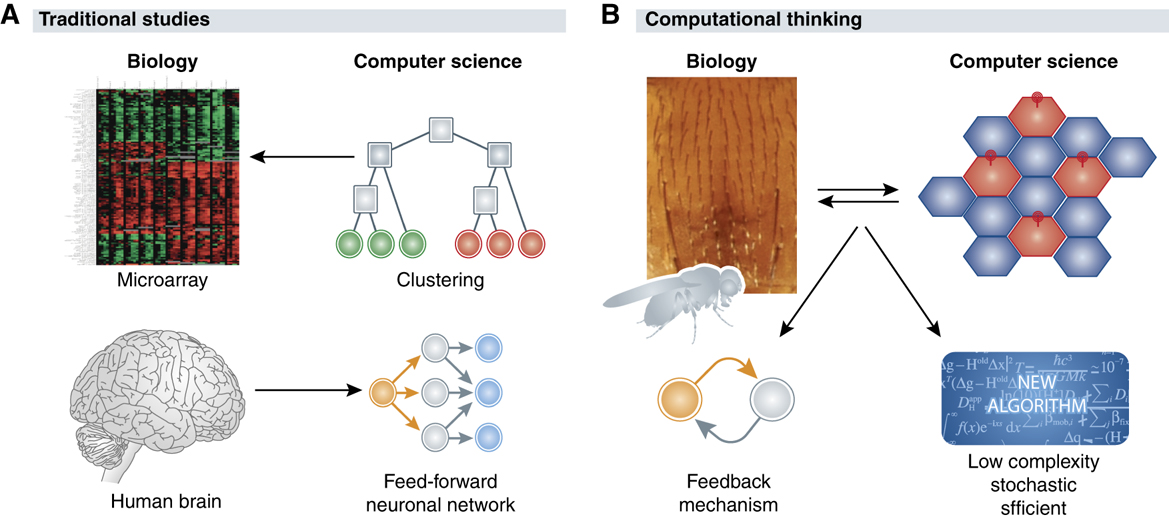
\includegraphics[width=0.9\textwidth]{new_images/nature-inspired.jpg}


%% Ref Fister jr, Iztok & Yang, Xin-She & Fister, Iztok & Brest, Janez & Fister, Du�an. (2013). A Brief Review of Nature-Inspired Algorithms for Optimization. Elektrotehniski Vestnik/Electrotechnical Review. 80.
\end{frame}
%-----------------------------------------------------------------------
%----------------------------------------------------------------------

%\begin{frame}[c]{Nature Inspired Algorithms for Optimization}
%\centering
%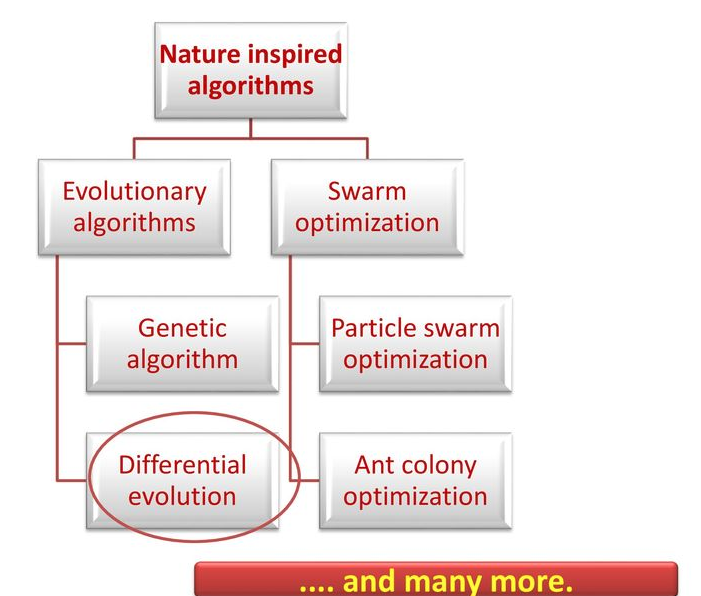
\includegraphics[width=0.7\textwidth]{new_images/nature-inspired-opt.png}
%\end{frame}
%-----------------------------------------------------------------------
%----------------------------------------------------------------------

\begin{frame}[c]{Nature Inspired Algorithms for Optimization \litw{Fister et al. 2013}}
\centering
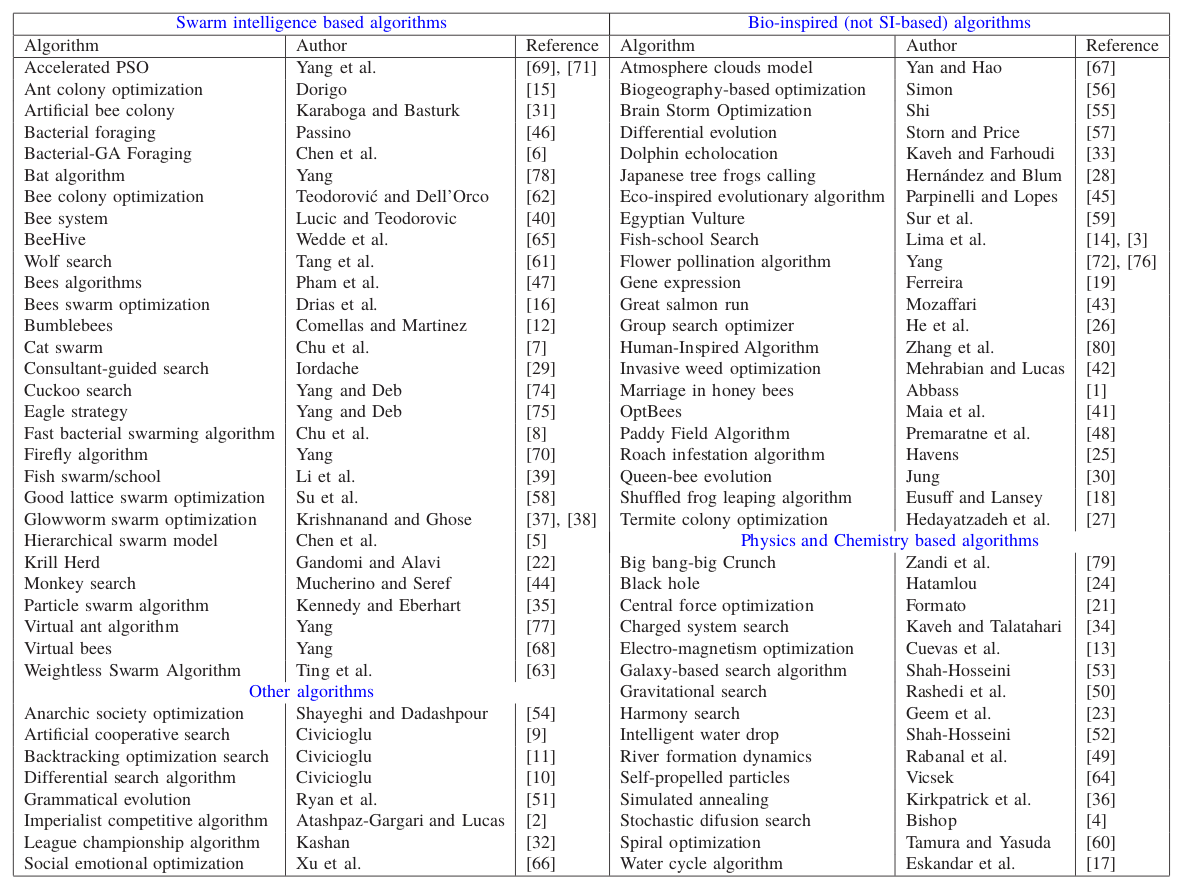
\includegraphics[width=0.9\textwidth]{new_images/nature-inspired-algs.png}
%% Ref Fister jr, Iztok & Yang, Xin-She & Fister, Iztok & Brest, Janez & Fister, Du�an. (2013). A Brief Review of Nature-Inspired Algorithms for Optimization. Elektrotehniski Vestnik/Electrotechnical Review. 80.
\end{frame}
%-----------------------------------------------------------------------
%----------------------------------------------------------------------

\begin{frame}[c]{Nature Inspired Algorithms for Optimization}
\begin{block}{Evolutionary Computation (EC)}
is a family of algorithms for global optimization inspired from biological evolution.
\begin{itemize}
    \item Evolutionary Algorithms (EAs) are subset of EC, and generic population-based optimization algorithms.
\end{itemize}
 
\end{block}
%\begin{minipage}{0.99\textwidth}
%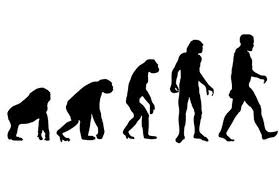
\includegraphics[width=\textwidth]{new_images/EAs0.jpeg}
%\end{minipage}
\centering
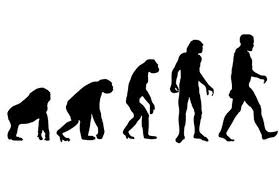
\includegraphics[width=0.6\textwidth]{new_images/EAs0.jpeg}
\end{frame}
%----------------------------------------------------------------------
\section{How Evolutionary Algorithms Work}
%----------------------------------------------------------------------

\begin{frame}[c]{How Evolutionary Algorithms Work}
\begin{itemize}
    \item Basic steps of an evolutionary algorithms are: 
    \begin{itemize}
        \item Initialization, Mutation, Recombination (Crossover), Selection
    \end{itemize}
\end{itemize}
\pause
\begin{center}
\begin{minipage}[c]{0.49\textwidth}
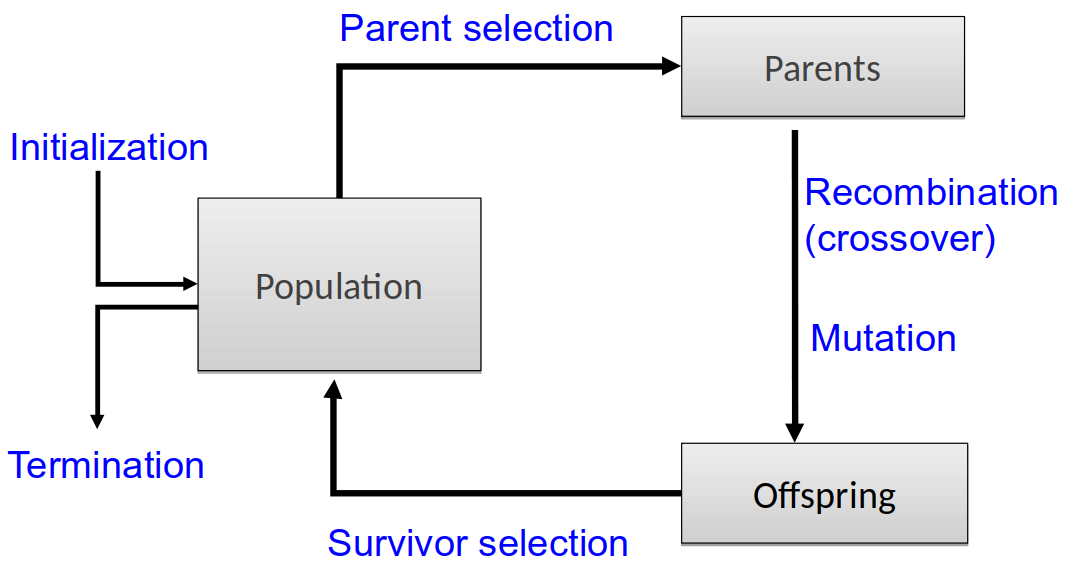
\includegraphics[width=\textwidth]{new_images/EAs1.png}
\end{minipage}
\begin{minipage}[c]{0.49\textwidth}
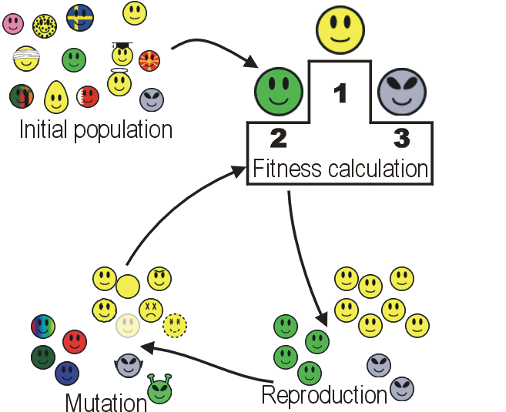
\includegraphics[width=\textwidth]{new_images/EAs4.png} 
\end{minipage}
\end{center}

\tiny{\lit{\href{https://www.brutalhack.com/blog/our-experiment-design/}{source}}}
\end{frame}
%----------------------------------------------------------------------
%----------------------------------------------------------------------

\begin{frame}[c,fragile]{How Evolutionary Algorithms Work}
\begin{algorithm}[H]
	\Input{black-box function $f$,
	    dimension $D$,
		maximal number of function evaluations $FE_{max}$,
		population size $NP$,
		mutation rate,
		crossover rate
	}
	\BlankLine
	$g$ = 0, $FE$ = 0;\\
	\pause
	$pop_g$ $\leftarrow$ initial\_population($NP$,$D$); \\
	$fitness_g$ $\leftarrow$ evaluate\_population($pop_g$); \\
	$FE$ = $NP$; \\
	\pause
	\While{($FE$ $<$ $FE_{max}$)}{
		mutate($pop_g$);\\
		$offspring_g$ $\leftarrow$ crossover($pop_g$);\\
		$fitness_g$ $\leftarrow$ evaluate\_population($offspring_g$); \\
		\pause
		$pop_{g+1}$,$fitness_{g+1}$ $\leftarrow$ select($pop_g$,$offspring_g$); \\
	    $g$ = $g$+1;\\
	}
	\Return{Best individual $X$ in $pop$ according to $fitness$}
	\caption{Optimization with EA}
\end{algorithm}


%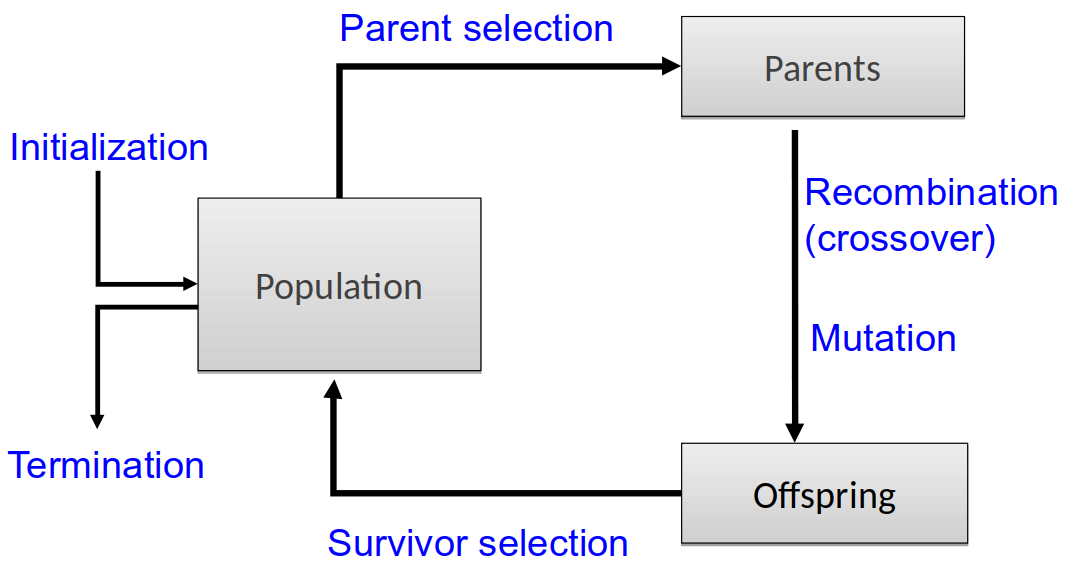
\includegraphics[width=6cm]{new_images/EAs1.png}

\end{frame}
%----------------------------------------------------------------------
%----------------------------------------------------------------------

\begin{frame}{How Evolutionary Algorithms Work}
\begin{center}
%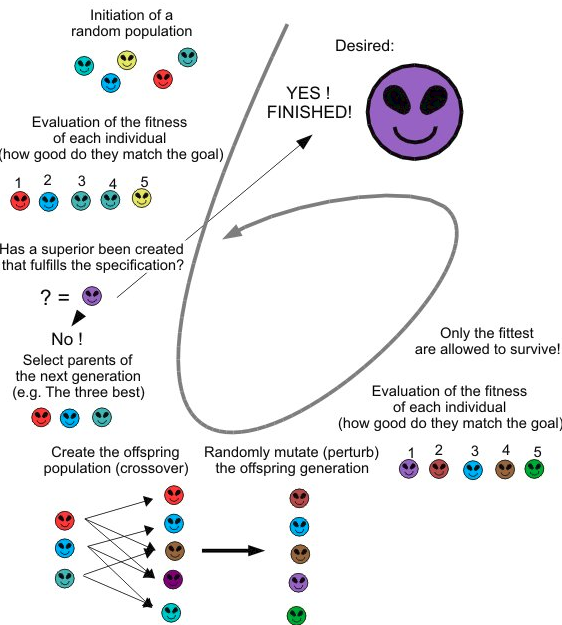
\includegraphics[width=6.9cm]{new_images/EAs55.png} 

\begin{block}{Representation}
Each individual is a solution of the problem being solved 
\begin{itemize}
    \item solutions are represented as vectors of size $D$ with each value taken from some domain
    \item each parameter $x_i$ in $X$ should be within the search range of the problem being solved [$Min$,$Max$]
\end{itemize}
\end{block}

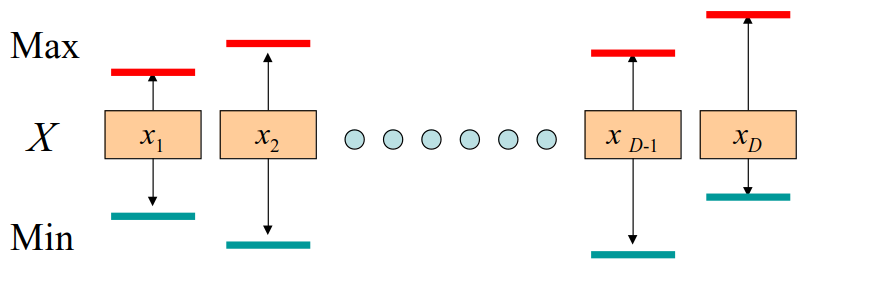
\includegraphics[width=9cm]{new_images/EAs_rep.png} 

\end{center}
\end{frame}
%----------------------------------------------------------------------
%----------------------------------------------------------------------

\begin{frame}{How Evolutionary Algorithms Work}
\begin{center}
\begin{block}{Maintain Population}
Maintain a population of size $NP$
\end{block}

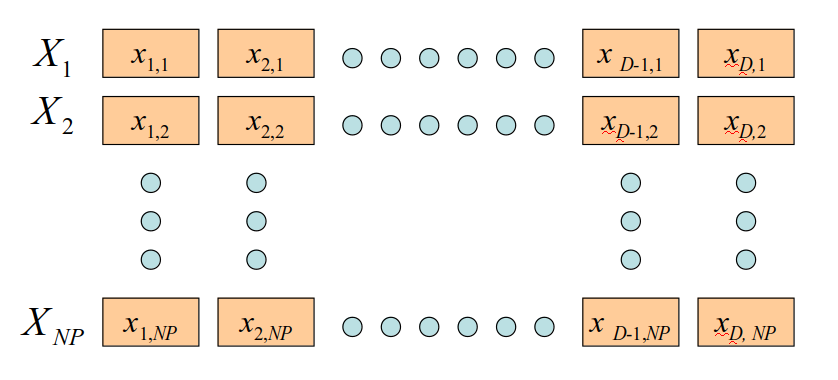
\includegraphics[width=9cm]{new_images/EAs_pop.png} 

\end{center}
\end{frame}
%----------------------------------------------------------------------
%----------------------------------------------------------------------

\begin{frame}{How Evolutionary Algorithms Work}
\begin{center}
\begin{block}{Maintain Population}
Maintain a population of size $NP$ 
\begin{itemize}
    \item initialize $NP$ $D$- dimensional individuals uniformly distributed within the search space 
    \item different $rand$ values are instantiated for each $i$ and $j$
\end{itemize}
\end{block}

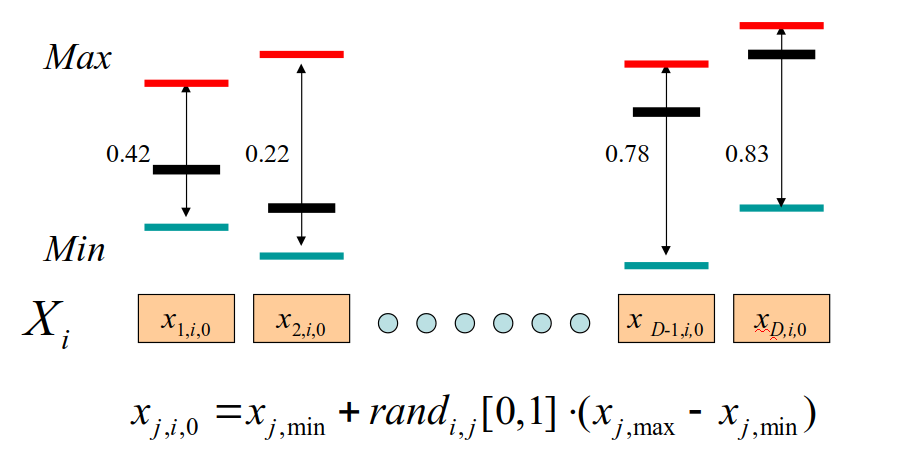
\includegraphics[width=9cm]{new_images/EAs_ini.png} 

\end{center}
\end{frame}
%----------------------------------------------------------------------
%----------------------------------------------------------------------

\begin{frame}{How Evolutionary Algorithms Work}
\begin{block}{Evolve Population}
Generate a new child (offspring) through mutation and crossover operations
\begin{itemize}
    \item mutation operation is to generate new mutant vector from the the current population/parents based on some criterion(strategy)   
    \item crossover operation is to combine the parent and mutant vector into one final offspring (i.e.\ inherit some features from parent and some from mutant vector)  
\end{itemize}
\end{block}
\centering
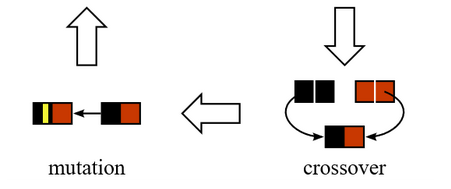
\includegraphics[width=0.5\textwidth]{new_images/pop00.png}
\end{frame}
%----------------------------------------------------------------------
%----------------------------------------------------------------------

\begin{frame}{How Evolutionary Algorithms Work}
\begin{block}{Parent Selection Mechanism}

"Survival of the fitter principle": each offspring is compared with its parent(s) and the one with a better fitness is forwarded to the next generation population
\begin{itemize}
    \item high quality solutions more likely to become parents than low quality
\end{itemize}
\end{block}
\centering
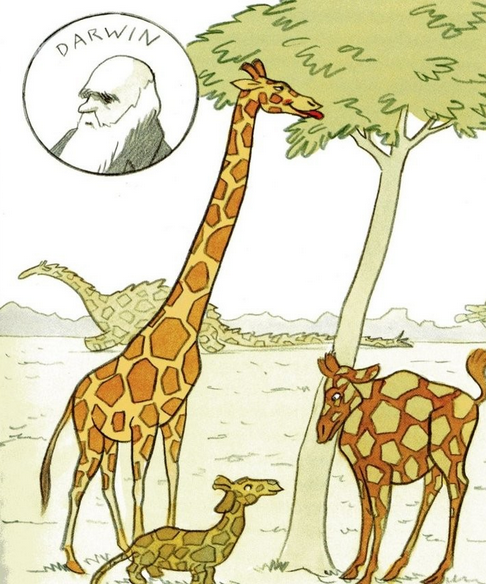
\includegraphics[width=0.35\textwidth]{new_images/selec00.png} 

\end{frame}
%----------------------------------------------------------------------
%----------------------------------------------------------------------
\begin{frame}{EAs Applied to HPO}
Task: \hands [2min] \linebreak
Why might EAs be an interesting approach for HPO and many other real-life applications?
\pause
\begin{itemize}
    \item very intuitive to use EAs for hyper-parameter tuning/optimization  
    \item can handle different data types
    %\item EAs has proven a powerful mechanism in improving life-forms and forming ever more complex species
    \item driven by surprisingly simple operations, nevertheless produced astonishing results
    \item time complexity is low compared to other model-based methods
    \begin{itemize}
        \item no need to fit a model and evaluate it performance on validation data, hence the process is not expensive like in BO
        \item parallelizable as a population of $N$ individuals can be evaluated in parallel on $N$ machines  
    \end{itemize}
\end{itemize}

\end{frame}
%----------------------------------------------------------------------
%----------------------------------------------------------------------

\begin{frame}{EAs Applied to HPO}
\begin{block}{General Concept}
We will generally define HPO problem as we wish to find the best combination of parameters that maximizes/minimizes some objective function (or fitness) by
\begin{itemize}
    \item define a population of $NP$ random individuals (or solutions) $\rightarrow$ $pop_{g0}$
    \item start the evolutionary search by evolving $pop_g$ using mutation (and/or) crossover $\rightarrow$ $popnew_g$
    \item survival of the fittest $\rightarrow$ best individuals is now $pop_{g+1}$  
    \item we will accept a final solution once we have either ran the algorithm for some maximum number of iterations, or we have reached some fitness threshold
\end{itemize}
\end{block}
\end{frame}
%----------------------------------------------------------------------
%----------------------------------------------------------------------

\begin{frame}{Evolutionary Algorithms}
\begin{block}{Pros and Cons of classical EAs}
Pros:
\begin{itemize}
    \item derivative-free methods
    \item can solve variety of optimization problems and real-world applications
    \pause
    \item highly parallelizable
    \item conceptually simple, yet powerful enough to solve complex problems
    \item time complexity is low compared to other algorithms
    \pause
\end{itemize}

Cons:
\begin{itemize}
    \item stagnation: optimization process does not progress anymore
    \item premature convergence: algorithm converges to a single solution, but that solution is not as high quality as expected
    \pause
    \item loss of population diversity for solving complex optimization problems
    \item lacks a good balance between exploration and exploitation 
\end{itemize}
\end{block}
\end{frame}

%----------------------------------------------------------------------
\section{Different Types of Evolutionary Algorithms}
%----------------------------------------------------------------------
\begin{frame}{Different Types of Evolutionary Algorithms}
Task: \hands [2min] \linebreak \linebreak
Although different EAs are similar at highest level, each of these varieties implements an EA in a different manner. What are the possible differences? 
\begin{center}
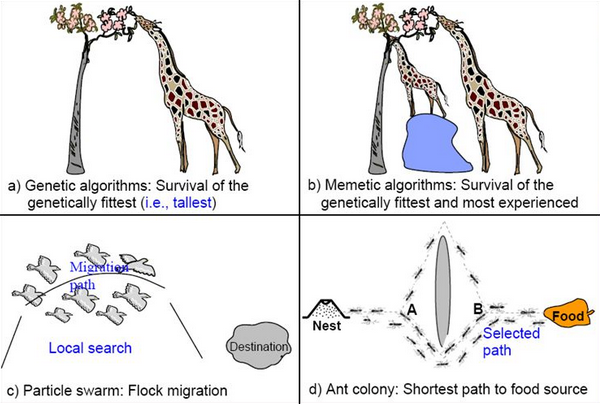
\includegraphics[width=0.6\textwidth]{new_images/EAs_03.png}
\end{center}

\end{frame}
%----------------------------------------------------------------------
%----------------------------------------------------------------------

\begin{frame}{Different Types of Evolutionary Algorithms}
Task: \hands [2min] \linebreak \linebreak
Although different EAs are similar at highest level, each of these varieties implements an EA in a different manner. What are the possible differences? \linebreak
The differences include almost all aspect of evolutionary search including:
\begin{itemize}
    \item Choices of representation for individual structures
    \item \textbf{Forms of mutation and crossover operations}
    \item Types of selection mechanism used
    \item Measures of performance
\end{itemize}
\end{frame}
%----------------------------------------------------------------------
%----------------------------------------------------------------------

%----------------------------------------------------------------------
%\subsection{Evolution Strategy (ES)}
%----------------------------------------------------------------------

\begin{frame}{Evolution Strategy (ES) \litw{Beyer and Schwefel. 2002}}
An optimization technique based on ideas of evolution.   
\begin{itemize}
    \item introduced in the early 1960s and then it developed further
    \item search operators are mutation and selection 
    \pause
    \item mutation operator adds a random number to each vector component, where the mutation rate or individual step size is usually governed by 
    \begin{itemize}
        \item self-adaptation mechanism uses multivariate normal distribution 
        \item covariance matrix adaptation (CMA-ES) 
        \pause
        \begin{itemize}
            \item represents the pairwise dependencies between the variables
            \item learns a second order model of the objective function using the ranking of candidate solutions (NOT the derivative nor function values are required)   
            
        \end{itemize}
    \end{itemize}
\end{itemize}
\begin{center}
%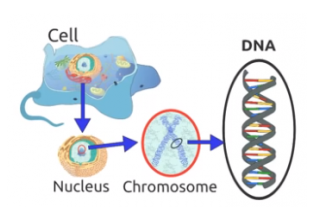
\includegraphics[width=0.5\textwidth]{new_images/GA_0.png}    
\end{center}

\end{frame}
%----------------------------------------------------------------------
%----------------------------------------------------------------------

\begin{frame}{Evolution Strategy (ES)}
Selection operator is based on fitness rankings, not actual fitness values  
\begin{itemize}
    \item $(1+\lambda)-$ES $ \rightarrow$ general ES rule in which $\lambda$ mutant vectors are generated and compete with the parent, and the best mutant becomes the parent for next generation
    \item $(1+1)-$ES $\rightarrow$ simplest ES
    \end{itemize}

\begin{center}
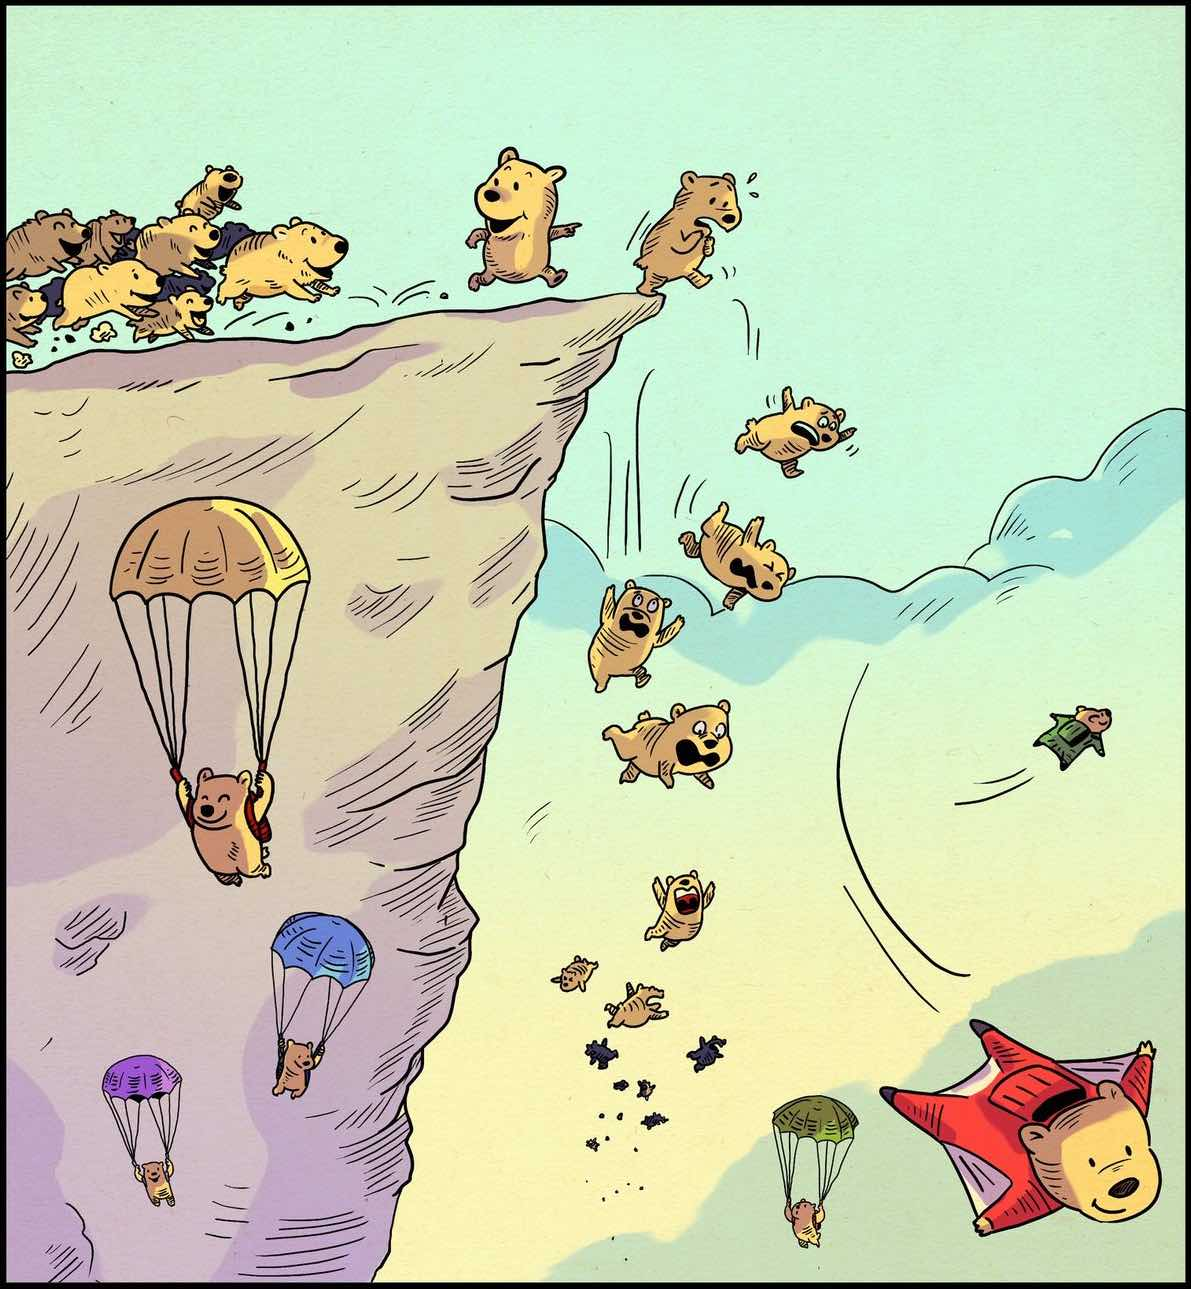
\includegraphics[width=6cm, height=4.5cm]{new_images/ES.jpeg}    
\end{center}

\end{frame}
%----------------------------------------------------------------------
%\subsection{Genetic Algorithm (GA)}
%----------------------------------------------------------------------

\begin{frame}{Genetic Algorithm (GA) \litw{Mitchell. 1998}}
The most popular type of EA which is inspired from the process of natural selection
\begin{itemize}
    \item introduced by Holland in 1960 based on the concept of Darwin's theory of evolution
    \item requires a genetic representation of the solution domain and a fitness function to evaluate the solution domain $\rightarrow$ encoding 
    \item applies genetic operators which are crossover and mutation (sometimes both, sometimes one)
\end{itemize}
\begin{center}
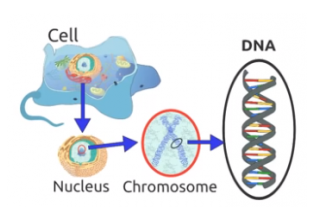
\includegraphics[width=0.5\textwidth]{new_images/GA_0.png}    
\end{center}

\end{frame}
%----------------------------------------------------------------------
%----------------------------------------------------------------------

\begin{frame}{How GA works}
\begin{minipage}[c]{0.59\textwidth}
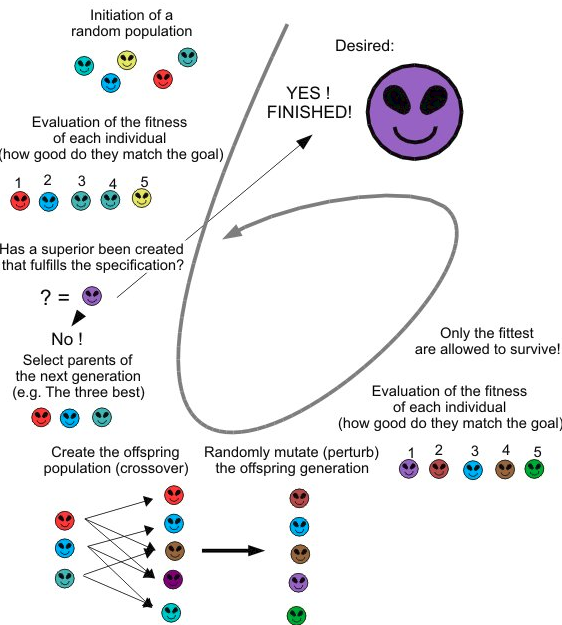
\includegraphics[width=\textwidth]{new_images/GA_1.png} \\~\\
\end{minipage}
%
\begin{minipage}[c]{0.3\textwidth}
Single-point crossover \\
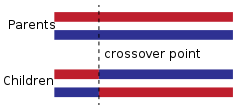
\includegraphics[width=4cm,height=2cm]{new_images/GA_3.png}\\~\\
Bit Flip mutation \\
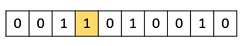
\includegraphics[width=4cm,height=0.6cm]{new_images/GA_mut1.png}\\
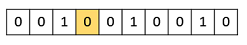
\includegraphics[width=4cm,height=0.6cm]{new_images/GA_mut2.png} \vspace{2.5cm}\\
\tiny{\lit{\href{https://www.kip.uni-heidelberg.de/vision/previous-projects/evolvable-hardware/evolutionary-algorithms/}{source}}}
\end{minipage}
\end{frame}
%----------------------------------------------------------------------
%\subsection{Differential Evolution (DE)}
%----------------------------------------------------------------------

\begin{frame}{Differential Evolution (DE) \litw{Storn and Price. 1995}}
One of the simplest, yet effective, stochastic direct search EA
\begin{itemize}
    \item introduced by Storn and Price in 1995
    \item outperformed several variants of GA and other EAs over a wide variety of optimization problems
    \item very easy to implement in any standard programming language
    \item very few control parameters (typically three for a standard DE) and their effects on the performance have been well studied
    \item complexity is very low as  compared to some of the most competitive continuous optimizers like CMA-ES
\end{itemize}
\end{frame}
%----------------------------------------------------------------------
%----------------------------------------------------------------------

\begin{frame}{How DE Works}
\centering
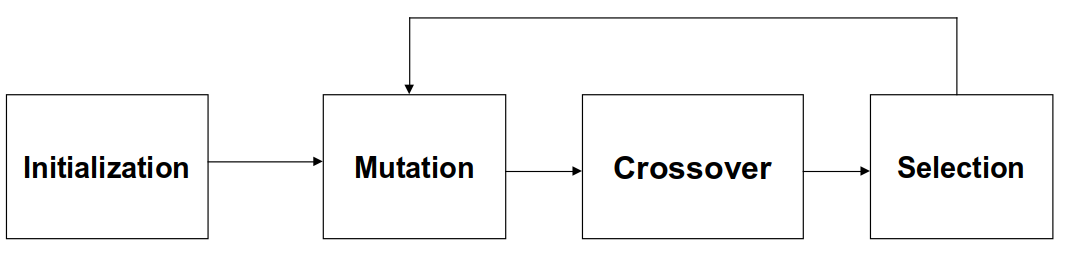
\includegraphics[width=1.0\textwidth]{new_images/DE1.png}\\
\end{frame}
%----------------------------------------------------------------------
%----------------------------------------------------------------------

\begin{frame}{Differential Evolution (DE)}
\centering
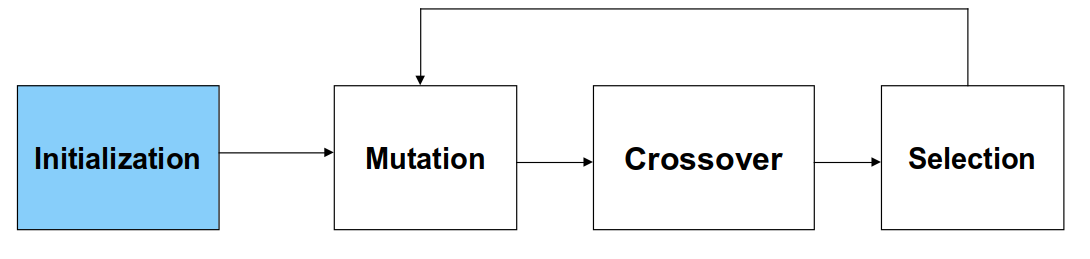
\includegraphics[width=1.0\textwidth]{new_images/DE2.png}\\
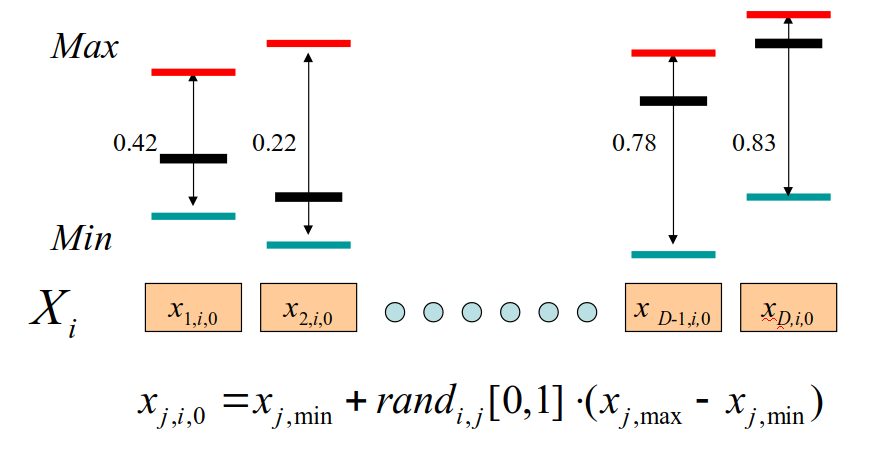
\includegraphics[width=0.7\textwidth]{new_images/DE3.png}\\
\end{frame}
%----------------------------------------------------------------------
%----------------------------------------------------------------------

\begin{frame}{Differential Evolution (DE)}
\centering
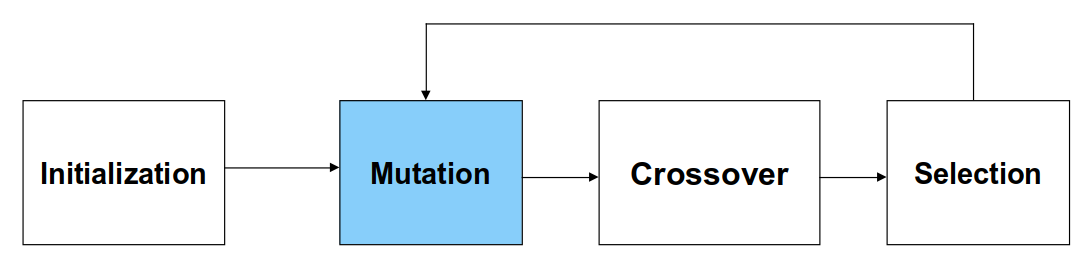
\includegraphics[width=1.0\textwidth]{new_images/DE4.png}\\
\begin{itemize}
    \item For each vector select three other parameter vectors randomly
    \item Add the weighted difference of two of the parameter vectors to the third to form a donor vector\\
    \begin{center}
        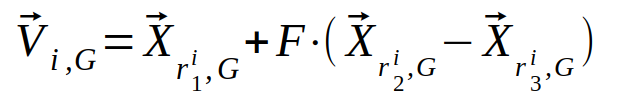
\includegraphics[width=0.5\textwidth]{new_images/DE5.png}
    \end{center}
    \item The scaling factor F is a random number from (0, 2)
\end{itemize}

\end{frame}
%----------------------------------------------------------------------
%----------------------------------------------------------------------

\begin{frame}{Differential Evolution (DE) \litw{Das and Suganthan. 2011}}
\centering
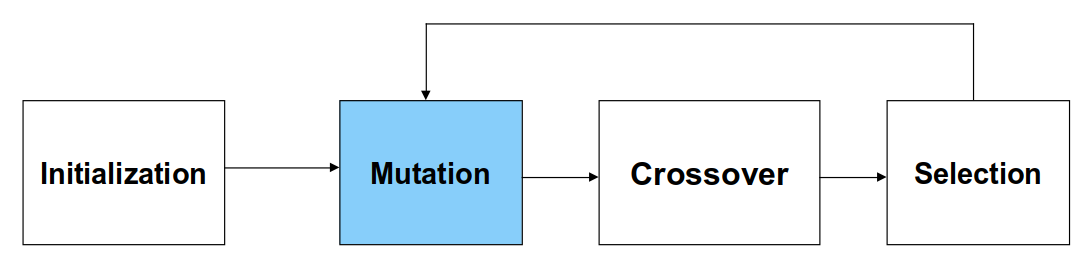
\includegraphics[width=1.0\textwidth]{new_images/DE4.png}\\
\begin{minipage}{0.43\textwidth}
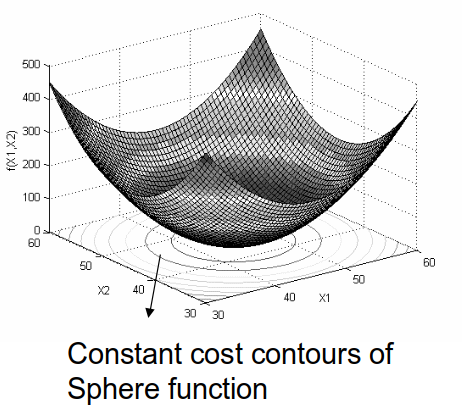
\includegraphics[width=\textwidth]{new_images/DE6.png}
\end{minipage}
\begin{minipage}{0.49\textwidth}
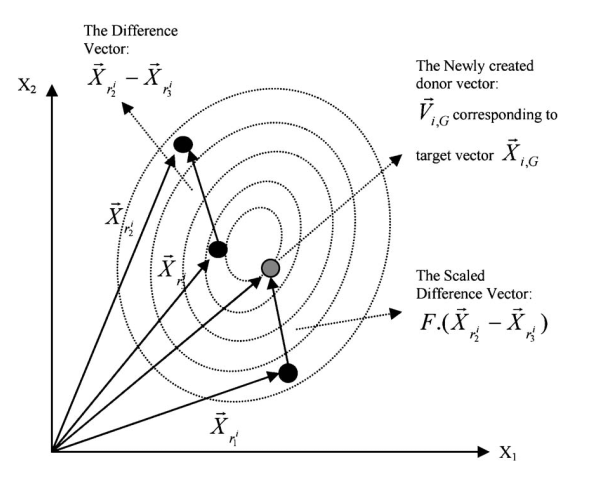
\includegraphics[width=\textwidth]{new_images/DE7.png}
\end{minipage}
\end{frame}
%----------------------------------------------------------------------
%----------------------------------------------------------------------

\begin{frame}{Differential Evolution (DE)}
\centering
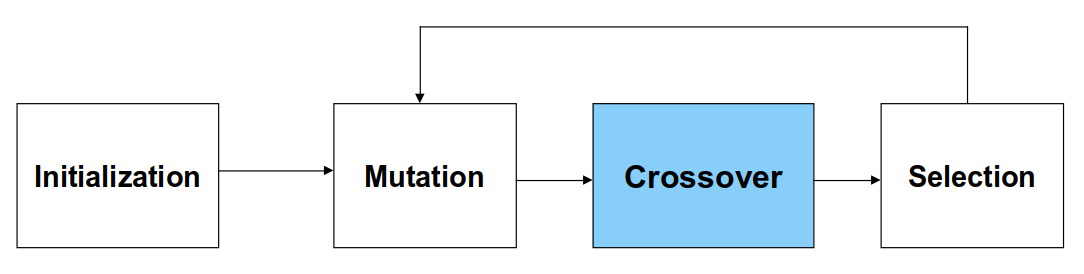
\includegraphics[width=1.0\textwidth]{new_images/DE8.png}\\
\begin{itemize}
    \item Binomial (Uniform) Crossover:
    \item Components of the donor vector enter into the trial offspring vector in the following way\\
    Let $j_{rand}$ be a randomly chosen integer between 1,...,$D$, and $CR$ is the crossover rate
\end{itemize}
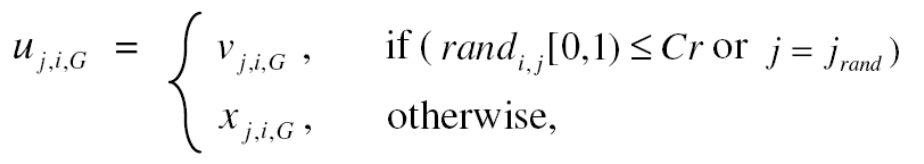
\includegraphics[width=0.7\textwidth]{new_images/DE9.png}\\
\end{frame}
%----------------------------------------------------------------------
%----------------------------------------------------------------------

\begin{frame}{Differential Evolution (DE)}
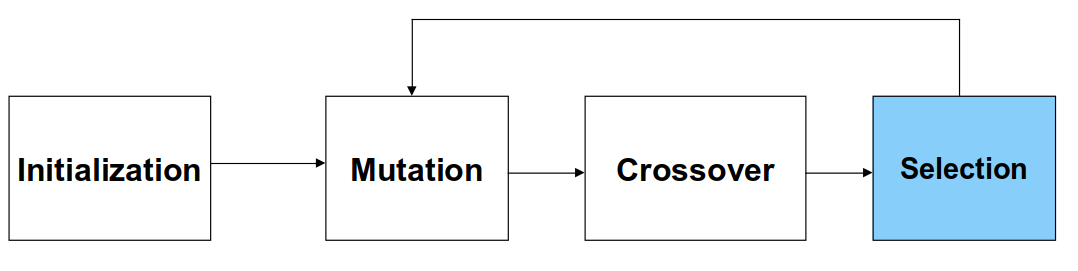
\includegraphics[width=1.0\textwidth]{new_images/DE10.png}\\~\\
\begin{itemize}
    \item "Survival of the fitter" principle \\
\end{itemize}
\centering
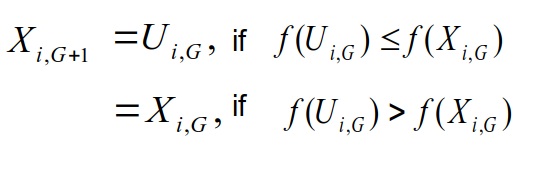
\includegraphics[width=0.5\textwidth]{new_images/EAs_selec.png}
\end{frame}
%----------------------------------------------------------------------
%----------------------------------------------------------------------

%----------------------------------------------------------------------
\section{EAs for Hyperparameter Optimization}
%----------------------------------------------------------------------
\begin{frame}{Tree-based Pipeline Optimization tool \litw{Olson et al. 2016}
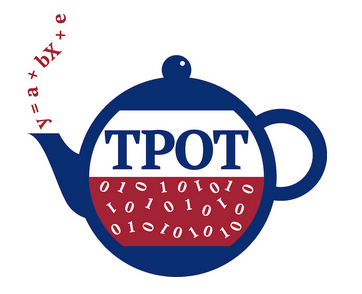
\includegraphics[width=0.1\textwidth]{new_images/TPOT.png}}
\begin{itemize}
    \item the very first AutoML method for hyperparameter tuning using genetic programming, and won the best paper award in GECCO 2016 
    \item \lit{\href{https://github.com/EpistasisLab/tpot}{GitHubTPOT}}: is built on top of scikit-learn
    \item automate the most tedious part of machine learning by intelligently exploring thousands of possible pipelines to find the best one for tested data 
\end{itemize}
\centering
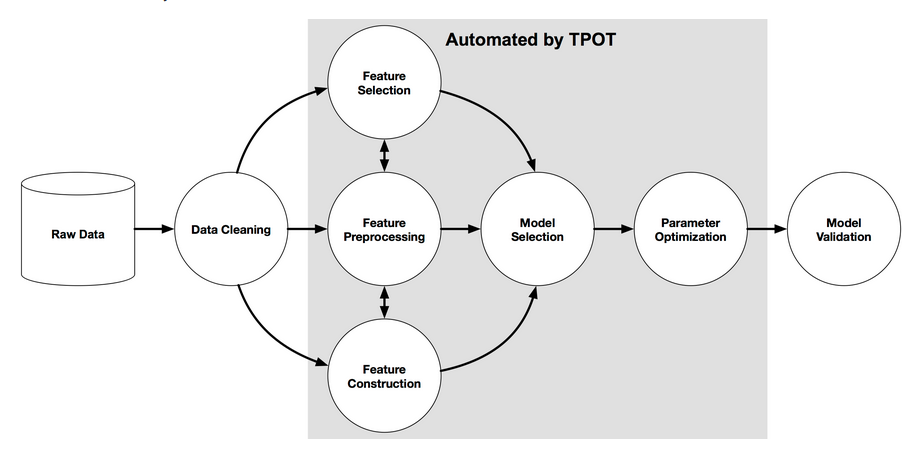
\includegraphics[width=0.75\textwidth]{new_images/tpot3.png}\\
\end{frame}
%----------------------------------------------------------------------
%----------------------------------------------------------------------

\begin{frame}{Tree-based Pipeline Optimization tool \litw{Olson et al. 2016}
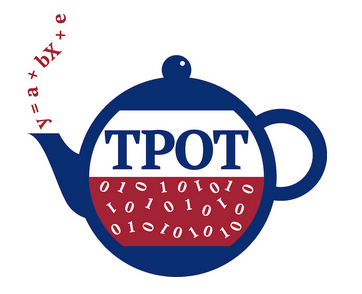
\includegraphics[width=0.1\textwidth]{new_images/TPOT.png}}
\begin{itemize}
    \item once evolutionary search is done, TPOT generates the best found pipeline as a Python code so you start from there \\~\\
\end{itemize}
\centering
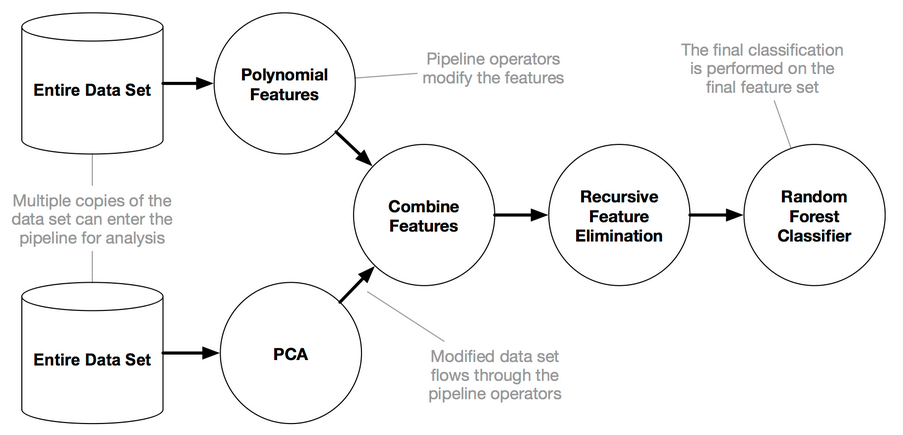
\includegraphics[width=0.8\textwidth]{new_images/tpot4.png}\\
\end{frame}
%----------------------------------------------------------------------
%----------------------------------------------------------------------

\begin{frame}{Neuroevolution \litw{Stanley 2017}}
\begin{itemize}
    \item is a ML technique that applies EAs to construct artificial neural networks (ANN), topology and rules. i.e.\ tuning NNs using EAs
    \item is highly general; it allows learning without explicit targets, with only sparse feedback, and with arbitrary neural models and network structures
    \item is an effective approach to solve reinforcement learning problems, and applied in evolutionary robotics and artificial life
\end{itemize}
\centering 
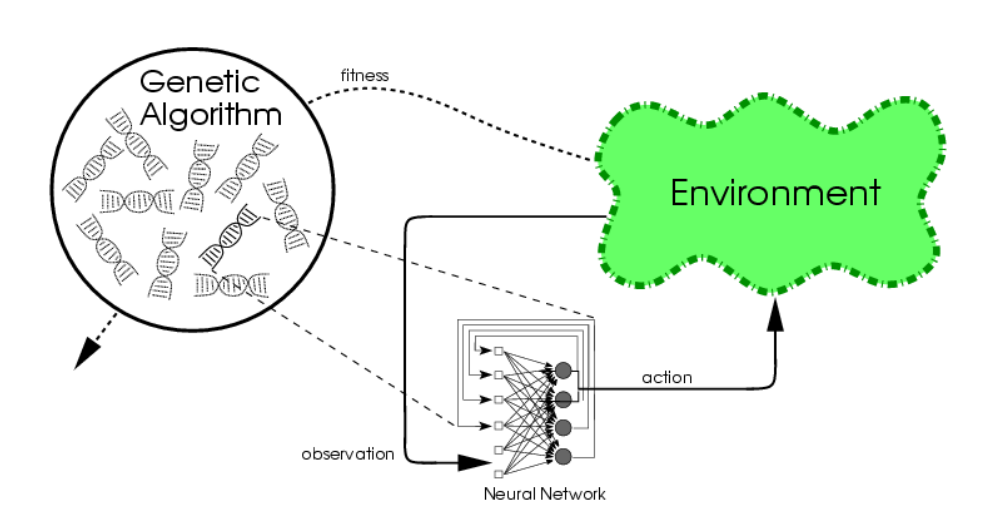
\includegraphics[width=0.7\textwidth]{new_images/neuroevo.png}
\end{frame}
%----------------------------------------------------------------------
%----------------------------------------------------------------------

\begin{frame}{Neuroevolution}
Different features for neuroevolution algorithms:
\begin{itemize}
    \item Conventional neuroevolution: evolve the weights for a fixed network topology 
    \item Topology and Weight Evolving Artificial Neural Network algorithms (TWEANNs): evolve both the topology of the network and its weights
    \item Evolve the structure of ANNs in parallel to its parameters or separately
\end{itemize}
\centering
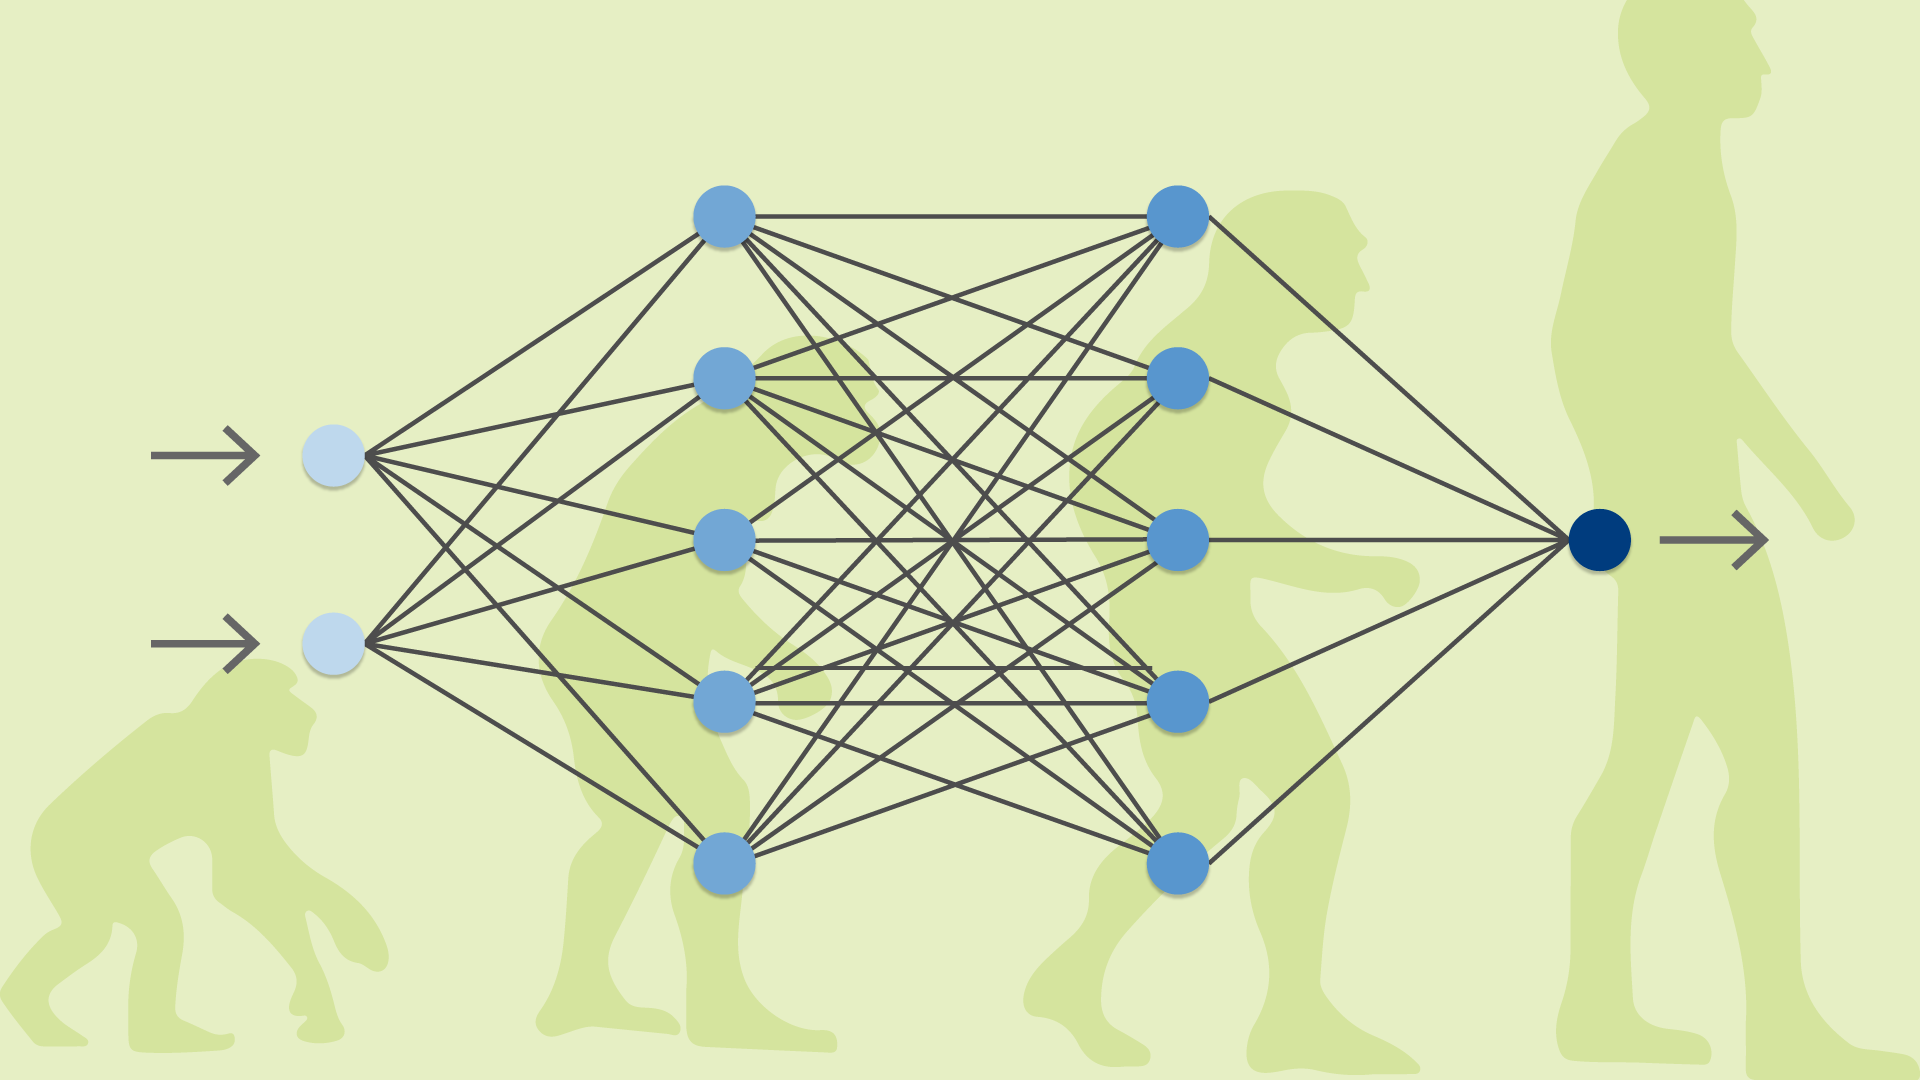
\includegraphics[width=0.7\textwidth]{new_images/NE1.png}
\end{frame}
%----------------------------------------------------------------------
%----------------------------------------------------------------------

\begin{frame}{Neuroevolution}
\begin{block}{Neuroevolution vs. Gradient descent}
Despite the fact that most NNs use gradient descent, neuroevolution are competitive with sophisticated modern gradient descent DL algorithms. Why?
\begin{itemize}
    \item because neuroevolution was found to be less likely to get stuck in local minimal. Many researchers at OpenAI and Uber proved that a simple neuroevolution algorithm is superior method  
    \item neuroevolution is succeeding where it had failed before due to the increased computational power available in the 2010s
    \item neuroevolution methods are powerful especially in continuous domains compared to reinforcement learning
\end{itemize}
\end{block}

\lit{\href{https://eng.uber.com/deep-neuroevolution/}{Welcoming the Era of Deep Neuroevolution}}
\end{frame}
%----------------------------------------------------------------------
%----------------------------------------------------------------------

\begin{frame}{Neuroevolution}
\begin{tabular}{||c|c|c|c||}
\hline
Method & Encoding & EAs & Aspects evolved \\ 
\hline\hline
     Neuro-genetic evolution 94 & Direct & GA & Network weights \\
     \hline
     Cellular Encoding (CE) 94 & Indirect & GP & Structure $\&$ parameters \\
     \hline
     EPNet 97 & Direct & EP & Structure $\&$ parameters \\
     \hline
     NEAT 2002 & Direct & GA & Structure $\&$ parameters \\
     \hline
     HyperNEAT 05/07 & Direct & ES & Structure $\&$ parameters \\
     \hline
     HyperNEAT 2008 & Indirect & GA & Structure $\&$ parameters \\
     \hline
     ES-HyperNEAT 2012 & Indirect & GA & Structure $\&$ parameters \\
     \hline
     ICONE 2012 & Direct & EA & Structure $\&$ parameters \\
     \hline
     . & . & . & . \\
     \hline
     . & . & . & . \\
     \hline
     CMA-HAGA 2017 & Direct & ES & Structure $\&$ weights \\
     \hline
     Deep-NE 2019 & Direct & GA & Structure $\&$ weights \\
     \hline
\end{tabular}
\\~\\
\lit{\href{https://www.nature.com/articles/s42256-018-0006-z}{Designing neural networks through neuroevolution, Nature Machine Intelligence, 2019}}
\end{frame}
%----------------------------------------------------------------------
%----------------------------------------------------------------------

\begin{frame}{What's More?}
\begin{itemize}
    \item ES to Play Atari Games/MuJoCo
    \begin{itemize}
        \item a simple algorithm, natural ES (NES) is introduced in 2017 as a scalable alternative to RL \lit{Salimans et al. 2017}
        \begin{itemize}
            \item performs competitively with the best deep reinforcement learning algorithms, including deep Q-networks (DQN) and policy gradient methods (A3C)
        \end{itemize}
        \item canonical ES, introduced in 2018, outperformed NES to play Atari games \lit{Chrabaszcz et al. 2018}
        \item evolves networks with 1.7 million parameters
    \end{itemize}
\end{itemize}
\centering
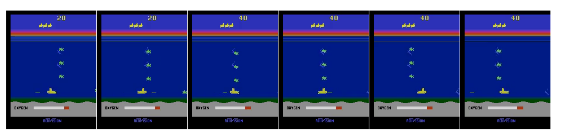
\includegraphics[width=0.7\textwidth]{new_images/ESA.png}\\
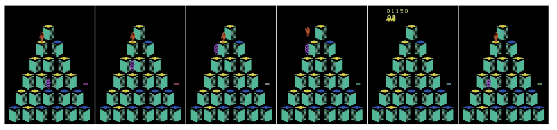
\includegraphics[width=0.7\textwidth]{new_images/ESA2.png}
\end{frame}
%----------------------------------------------------------------------
%----------------------------------------------------------------------

\begin{frame}{What's More?}
\begin{itemize}
    \item Large-scale evolution of image classifiers \lit{Real et al. 2017}
    \begin{itemize}
        \item the use of a simple EA to discover good models for CIFAR-10 and CIFAR-100 datasets, and reach high accuracies of around 95.6$\%$ and 77.0$\%$ respectively. 
    \end{itemize}
    \item HPO of DNNs using CMA-ES \lit{Loshchilov and Hutter 2016}
    \begin{itemize}
        \item tuned the hyperparameters of a convolutional neural network for the MNIST dataset of 19 hyperparameters, and outperformed state-of-the-art BO methods
    \end{itemize}
    \item Deep Neuroevolution \lit{Such et al. 2018}
    \begin{itemize}
        \item GAs are competitive alternative for training DNNs for RL
        \item evolves DNNs with a simple GA that performs well on hard deep RL problems (Atari game)
        \item GA performs as well as ES and deep RL algorithms based on DQN and A3C
        \item evolves networks with over four million parameters, the largest NNs ever evolved with a traditional EA
    \end{itemize}
\end{itemize}
\end{frame}
%----------------------------------------------------------------------
%----------------------------------------------------------------------

\begin{frame}{What's More?}
\begin{itemize}
    \item Evolutionary Robotics (ER)
    \begin{itemize}
        \item research field which uses EAs to develop hardware, controllers and strategies for autonomous robots. 
        \item population consists of candidate controllers which may be drawn from ANNs
        \item goal is to use the evolutionary search to evolve population and generate the best so-found controller using mutation and crossover operations
    \end{itemize}
\end{itemize}
\begin{minipage}[c]{0.49\textwidth}
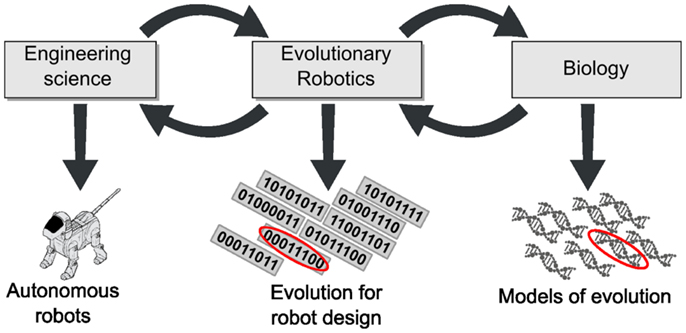
\includegraphics[width=\textwidth]{new_images/ER1.jpg}
\end{minipage}
\begin{minipage}[c]{0.49\textwidth}
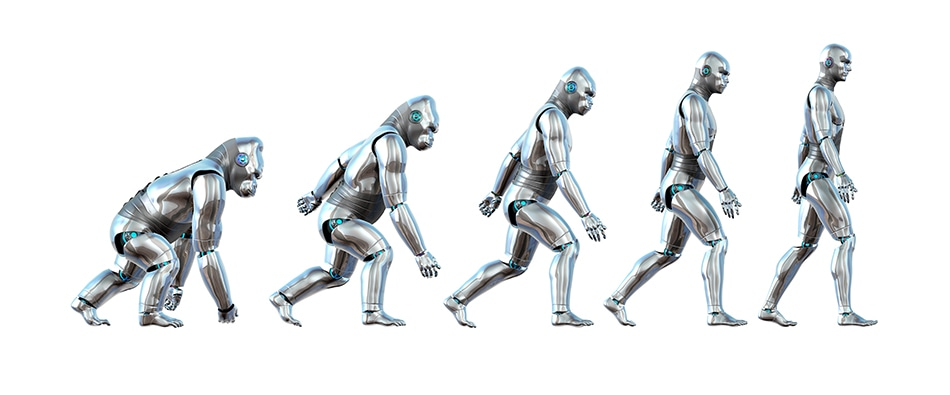
\includegraphics[width=\textwidth]{new_images/ER2.jpg} 
\end{minipage}
\linebreak
\begin{itemize}
    \item A very useful link about \lit{\href{http://www.evolutionaryrobotics.org/}{ER}}
\end{itemize}
\end{frame}

%----------------------------------------------------------------------
\section{Practical Considerations}
%----------------------------------------------------------------------
\begin{frame}{Challenges in EAs}
\begin{itemize}
    \item Classical EAs are sensitive to control hyperparameters setting
    \begin{itemize}
        \item for some EAs, the performance is highly dependent on the settings of mutation rate, crossover rate and population size 
    \end{itemize}
    \item Many researchers tackle this problem by developing successful \alert{self-adaptive mechanisms} for control parameter settings 
    \begin{itemize}
        \item adapt the settings of mutation and crossover rates using mathematical distributions such as: Cauchy, Normal, ... etc 
    \end{itemize}
\end{itemize}
\begin{center}
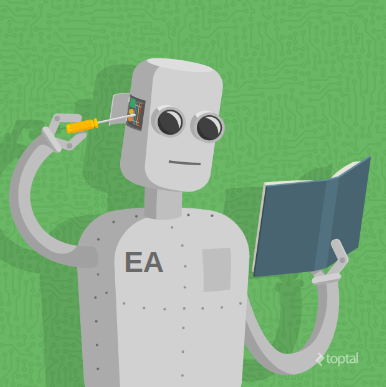
\includegraphics[width=0.38\textwidth]{new_images/EAc.png}
\end{center}    
\end{frame}
%----------------------------------------------------------------------
%----------------------------------------------------------------------

\begin{frame}{General Remark}
\begin{block}{No Free Lunch Theorem- NFL}
Over a large set of  problems, it is impossible to find a single best algorithm!
\end{block} \\~\\
\begin{minipage}[c]{0.49\textwidth}
\begin{itemize}
    \item for each specific problem there are suitable candidate algorithms
    \item you have to study and test them to know which one is the best fit for your problem
    \item you have to fine tune the algorithm's hyperparameters before you judge which one is the best
\end{itemize}
\end{minipage}
\begin{minipage}[c]{0.49\textwidth}
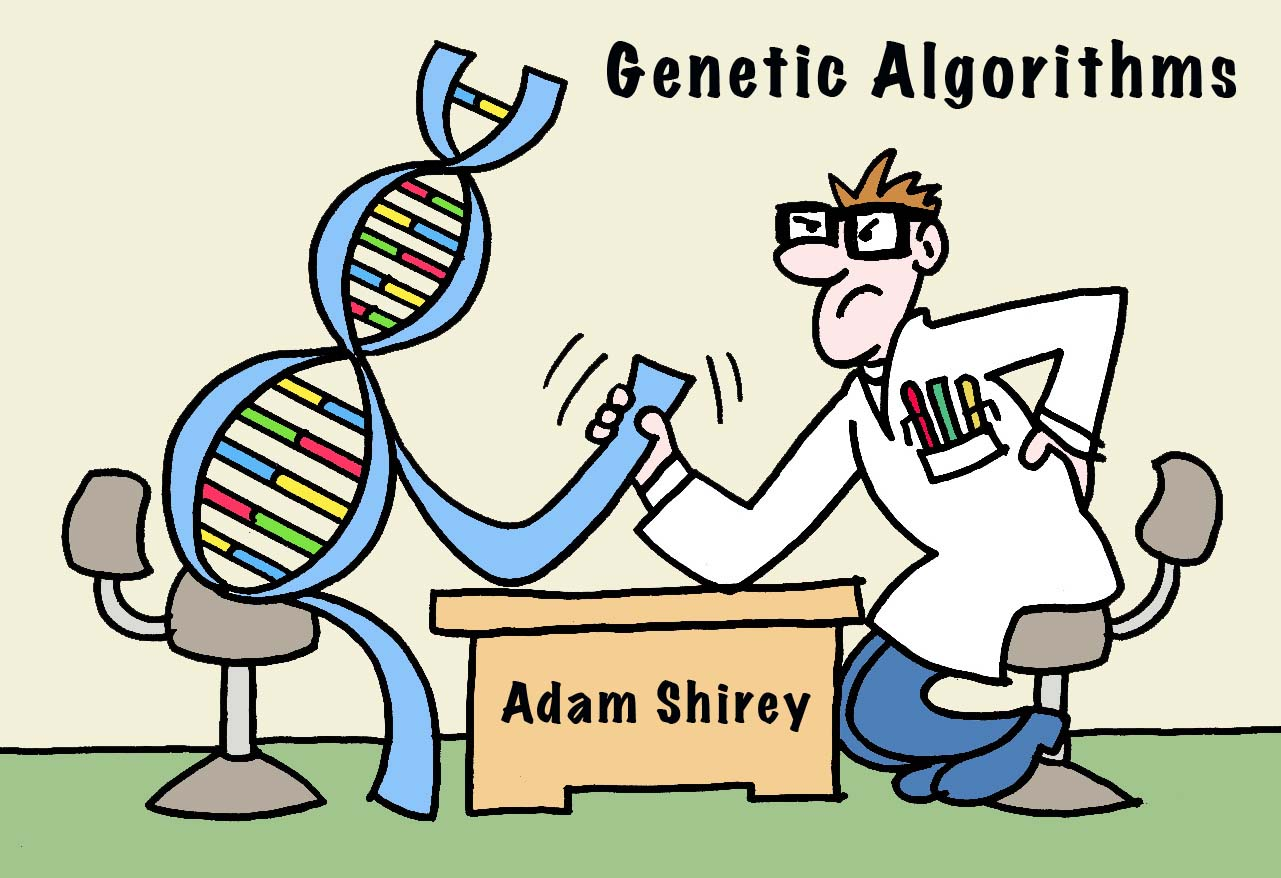
\includegraphics[width=\textwidth]{new_images/end1.jpg}
\end{minipage}
\end{frame}
%----------------------------------------------------------------------
%----------------------------------------------------------------------

\begin{frame}{General Remark}
Do you like evolutionary algorithms as much as I do? \hands \\~\\
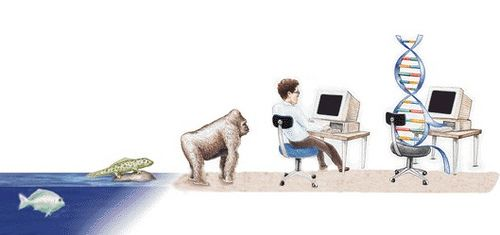
\includegraphics[width=\textwidth]{new_images/end2.jpg}
\end{frame}
%----------------------------------------------------------------------
%----------------------------------------------------------------------

\begin{frame}[c]{Learning Goals}
Now, you are able to \ldots

\begin{itemize}
	\item explain the basics of \alert{evolutionary algorithms}
	\item discuss the \alert{different types of evolutionary algorithms}
	\item efficiently tune \alert{HPO using evolutionary algorithms}
	\item discuss importance of \alert{evolutionary algorithms to solve many optimization problems}
\end{itemize}
\end{frame}
%----------------------------------------------------------------------
%----------------------------------------------------------------------

\begin{frame}[c]{Literature [These are links]}
\begin{itemize}
	\item \lit{\href{https://www.researchgate.net/publication/249645112_A_Brief_Review_of_Nature-Inspired_Algorithms_for_Optimization}{A Brief Review of Nature-Inspired Algorithms for Optimization. Fister et al. 2013}}
	
	\item \lit{\href{https://link.springer.com/article/10.1023/A:1015059928466}{Beyer and Schwefel. 2002. Evolution strategies � A comprehensive introduction}}
	
	\item \lit{\href{http://blog.otoro.net/2017/10/29/visual-evolution-strategies/}{Evolution Strategy}}
	
	\item \lit{\href{http://www.boente.eti.br/fuzzy/ebook-fuzzy-mitchell.pdf}{Mitchell. 1998. An Introduction to Genetic Algorithms}}
	
	\item \lit{\href{http://www1.icsi.berkeley.edu/~storn/code.html}{Storn and Price. 1995. Differential Evolution}}
	
	\item \lit{\href{https://ieeexplore.ieee.org/document/5601760}{Das and Suganthan. 2011. Differential Evolution}}
	
	\item \lit{\href{http://www1.icsi.berkeley.edu/~storn/code.html}{Storn and Price. 1995. Differential Evolution}}
	
	\item \lit{\href{https://link.springer.com/chapter/10.1007/978-3-319-31204-0_9}{Olson et al. 2016. TPOT}}
	
	\item \lit{\href{https://github.com/EpistasisLab/tpot}{GitHubTPOT}}
	
\end{itemize}

\end{frame}
%----------------------------------------------------------------------
%----------------------------------------------------------------------

\begin{frame}[c]{Literature [These are links]}
\begin{itemize}
	
	\item \lit{\href{https://www.oreilly.com/ideas/neuroevolution-a-different-kind-of-deep-learning}{Stanley 2017. Neuroevolution: A different kind of deep learning}}
	
	\item \lit{\href{https://arxiv.org/abs/1703.03864}{Salimans et al. 2017. Evolution Strategies as a Scalable Alternative to Reinforcement Learning}}
	
	\item \lit{\href{https://www.ijcai.org/proceedings/2018/0197.pdf}{Chrabaszcz et al. 2018. Back to Basics: Benchmarking Canonical Evolution Strategies for Playing Atari}}
	
	\item \lit{\href{https://arxiv.org/abs/1703.01041}{Real et al. 2017. Large-Scale Evolution of Image Classifiers}}
	
	\item \lit{\href{https://arxiv.org/pdf/1604.07269.pdf}{Loshchilov and Hutter 2016. CMA-ES for Hyperparameter Optimization of Deep Neural Networks}}
	
	\item \lit{\href{https://arxiv.org/abs/1712.06567}{Such et al. 2018. CDeep Neuroevolution}}
	
	 \item \lit{\href{http://www.evolutionaryrobotics.org/}{Evolutionary Robotics}}
	
\end{itemize}

\end{frame}